\renewcommand{\figurename}{Rys.}

\chapter*{Dodatek A}
\label{cha:dodatekA}
\addcontentsline{toc}{chapter}{Dodatek A}


\fontsize{14}{15}\selectfont
%----------------------------------------------------------
\begin{itemize}
	\item \textbf{Schematy elektryczne pulsoksymetru}
		\begin{itemize}
			\item Schemat~I  - układ sterowania intensywnością promieniowania diod LED,
			\item Schemat~II - konwerter prąd~-~napięcie i~układ  próbkująco~-~pamiętający,
			\item Schemat III - filtr dolnoprzepustowy Sallen~-~Key IV~rzędu,
			\item Schemat IV - mikrokontroler STM32, interfejs USB,
			\item Schemat V  - układ zasilania, interfejs JTAG .
		\end{itemize}
	\item \textbf{Projekt PCB}
		\begin{itemize}
			\item Warstwa TOP
			\item Warstwa BOTTOM
		\end{itemize}
	\item \textbf{Spis elementów w formie raportu BOM}
	\item \textbf{Raport symulacji filtru Bessela FilterPro TI}
\end{itemize}

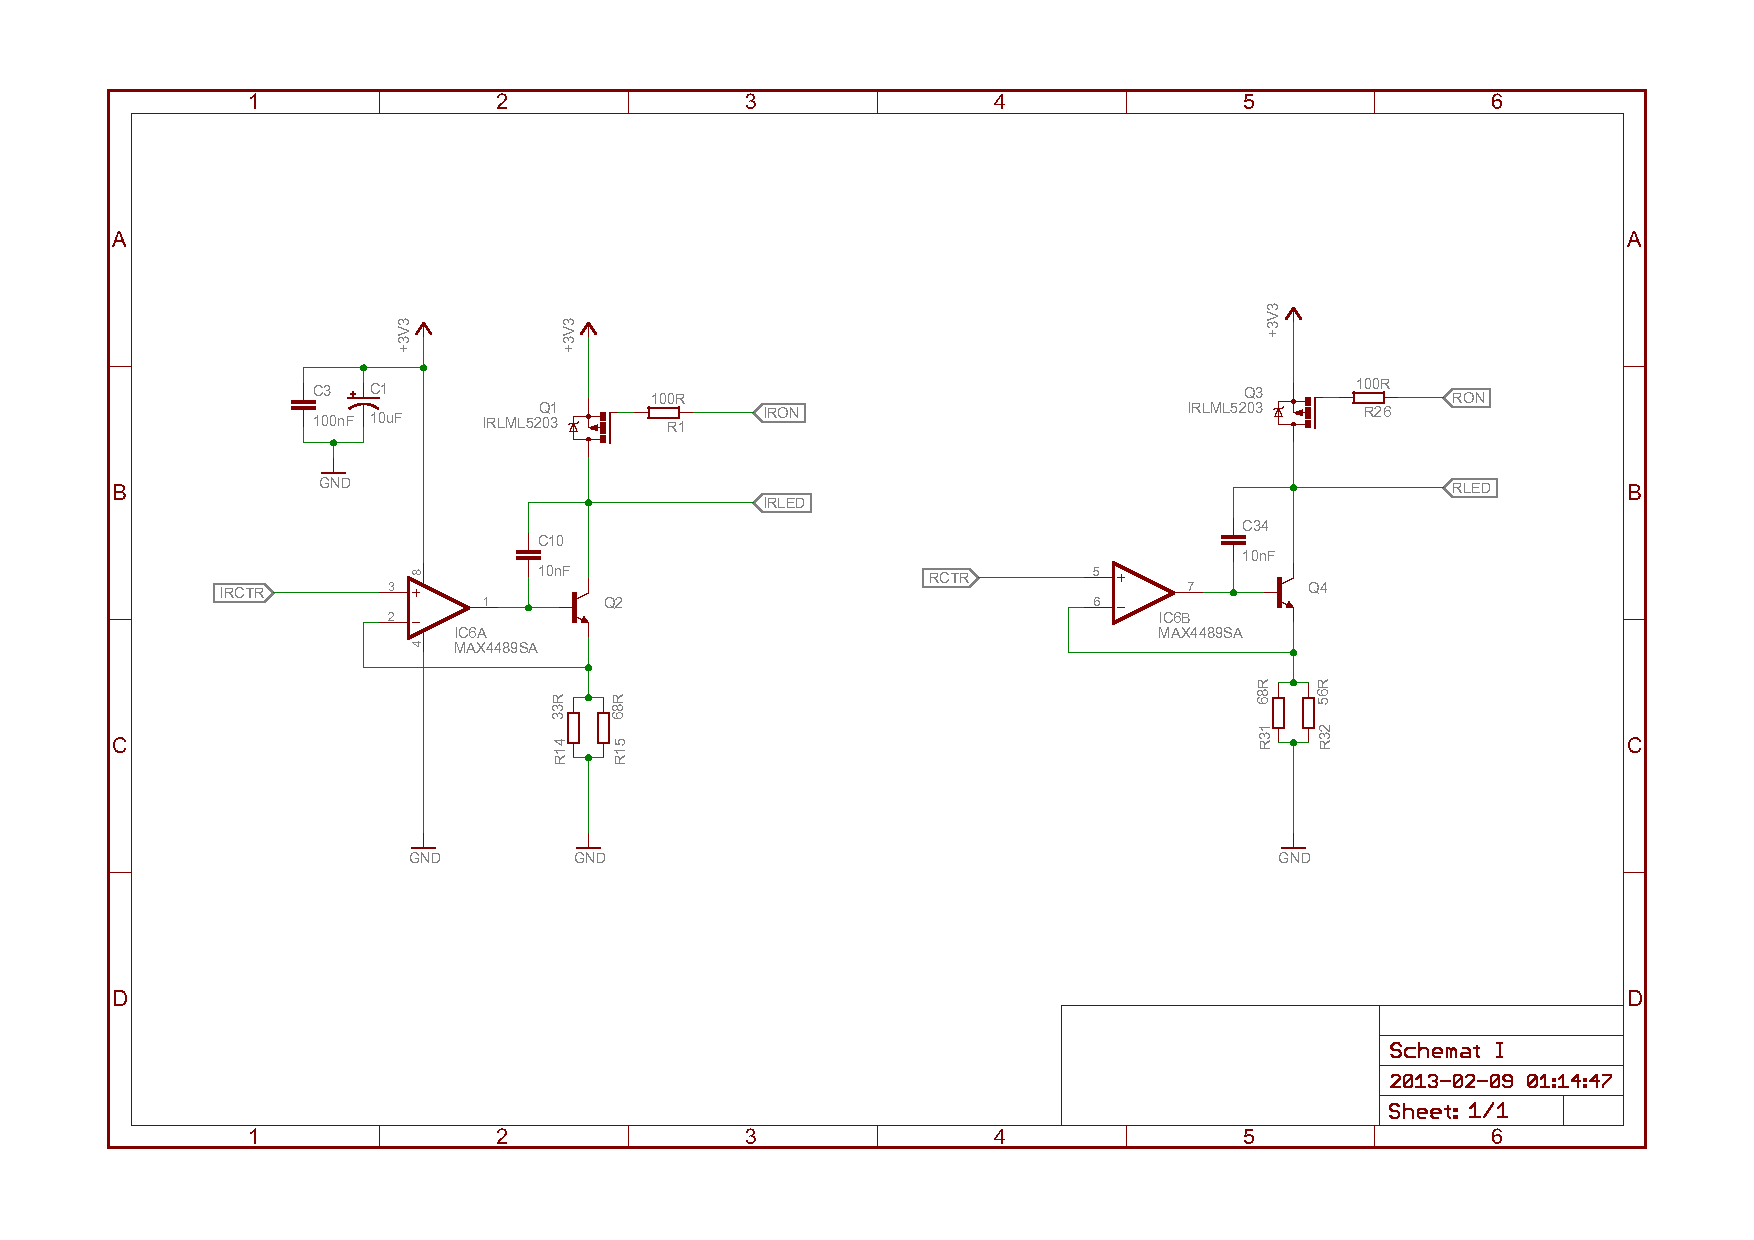
\includepdf[pages={1}, landscape]{graphic/SchematI.pdf}
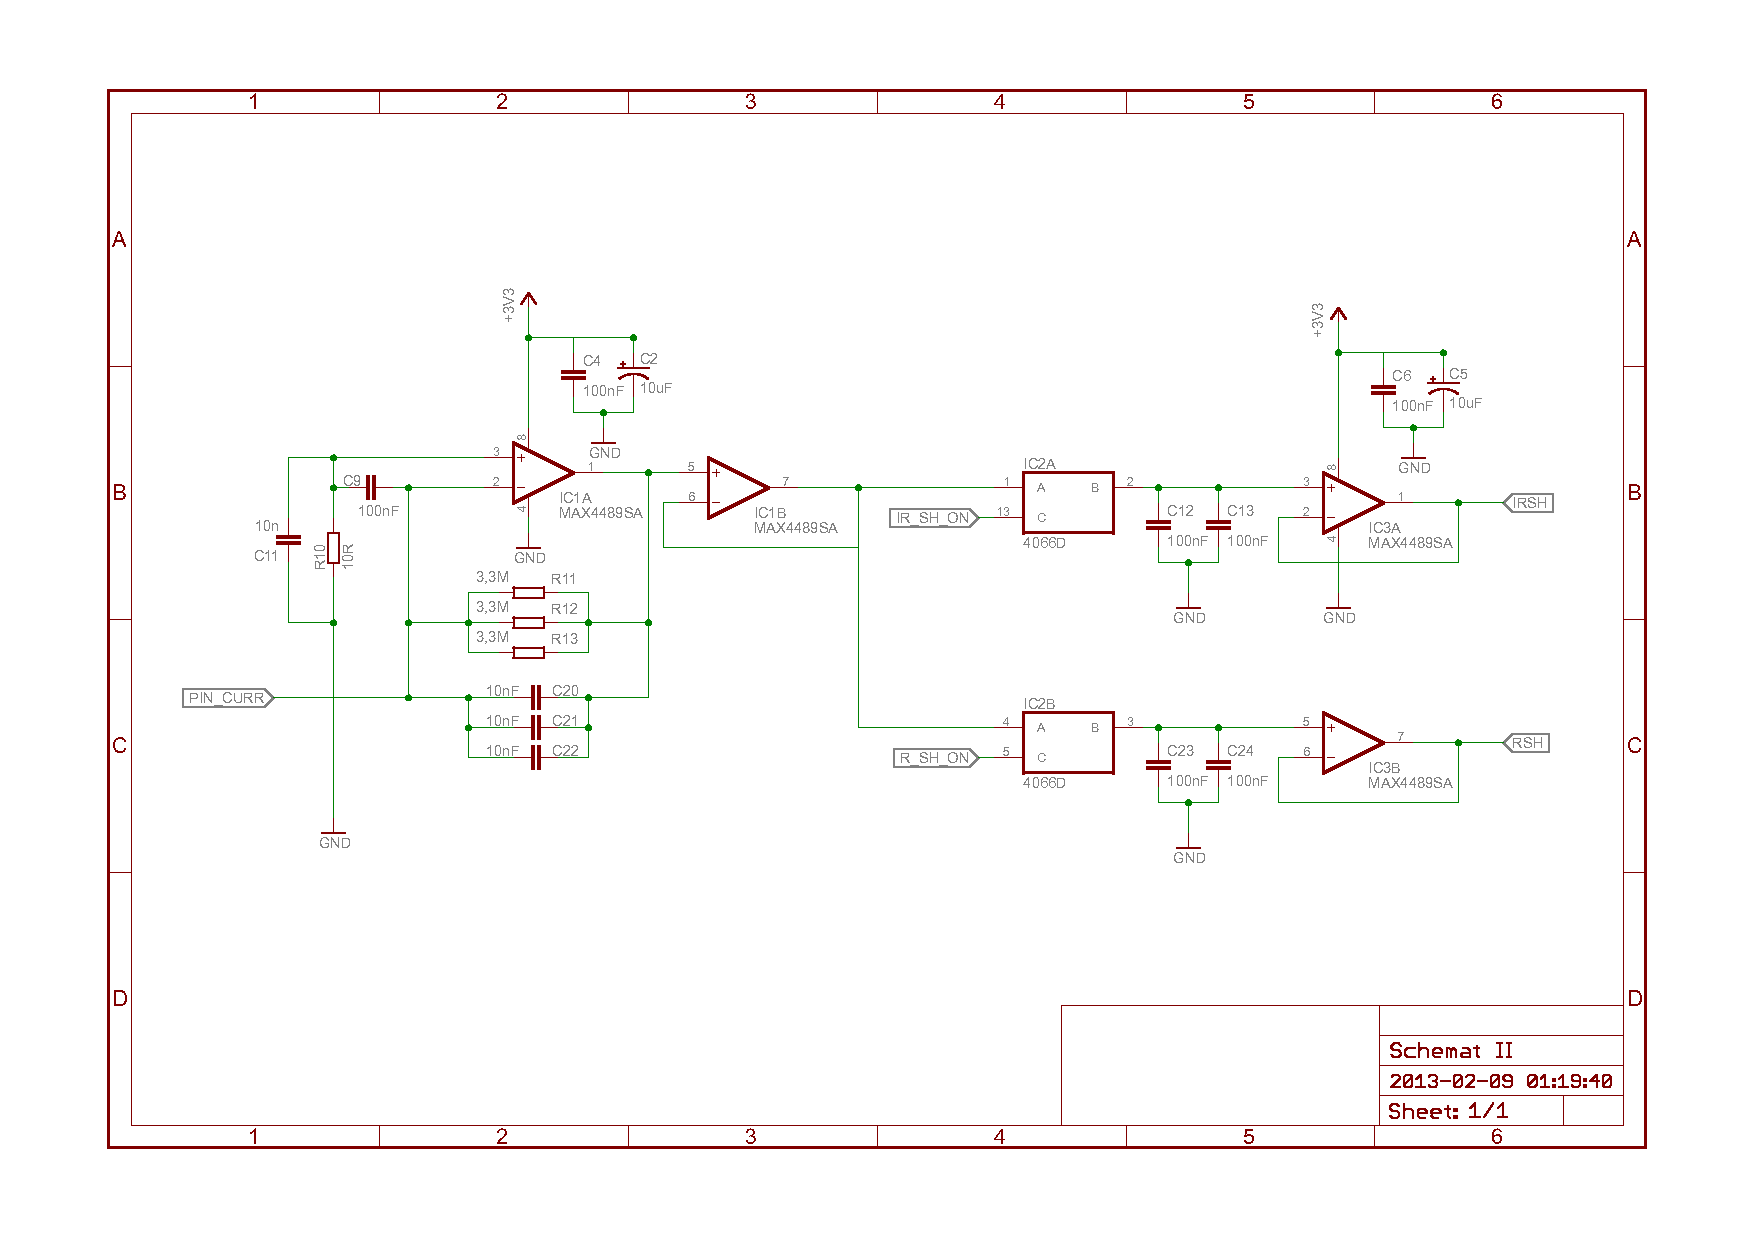
\includepdf[pages={1}, landscape]{graphic/SchematII.pdf}
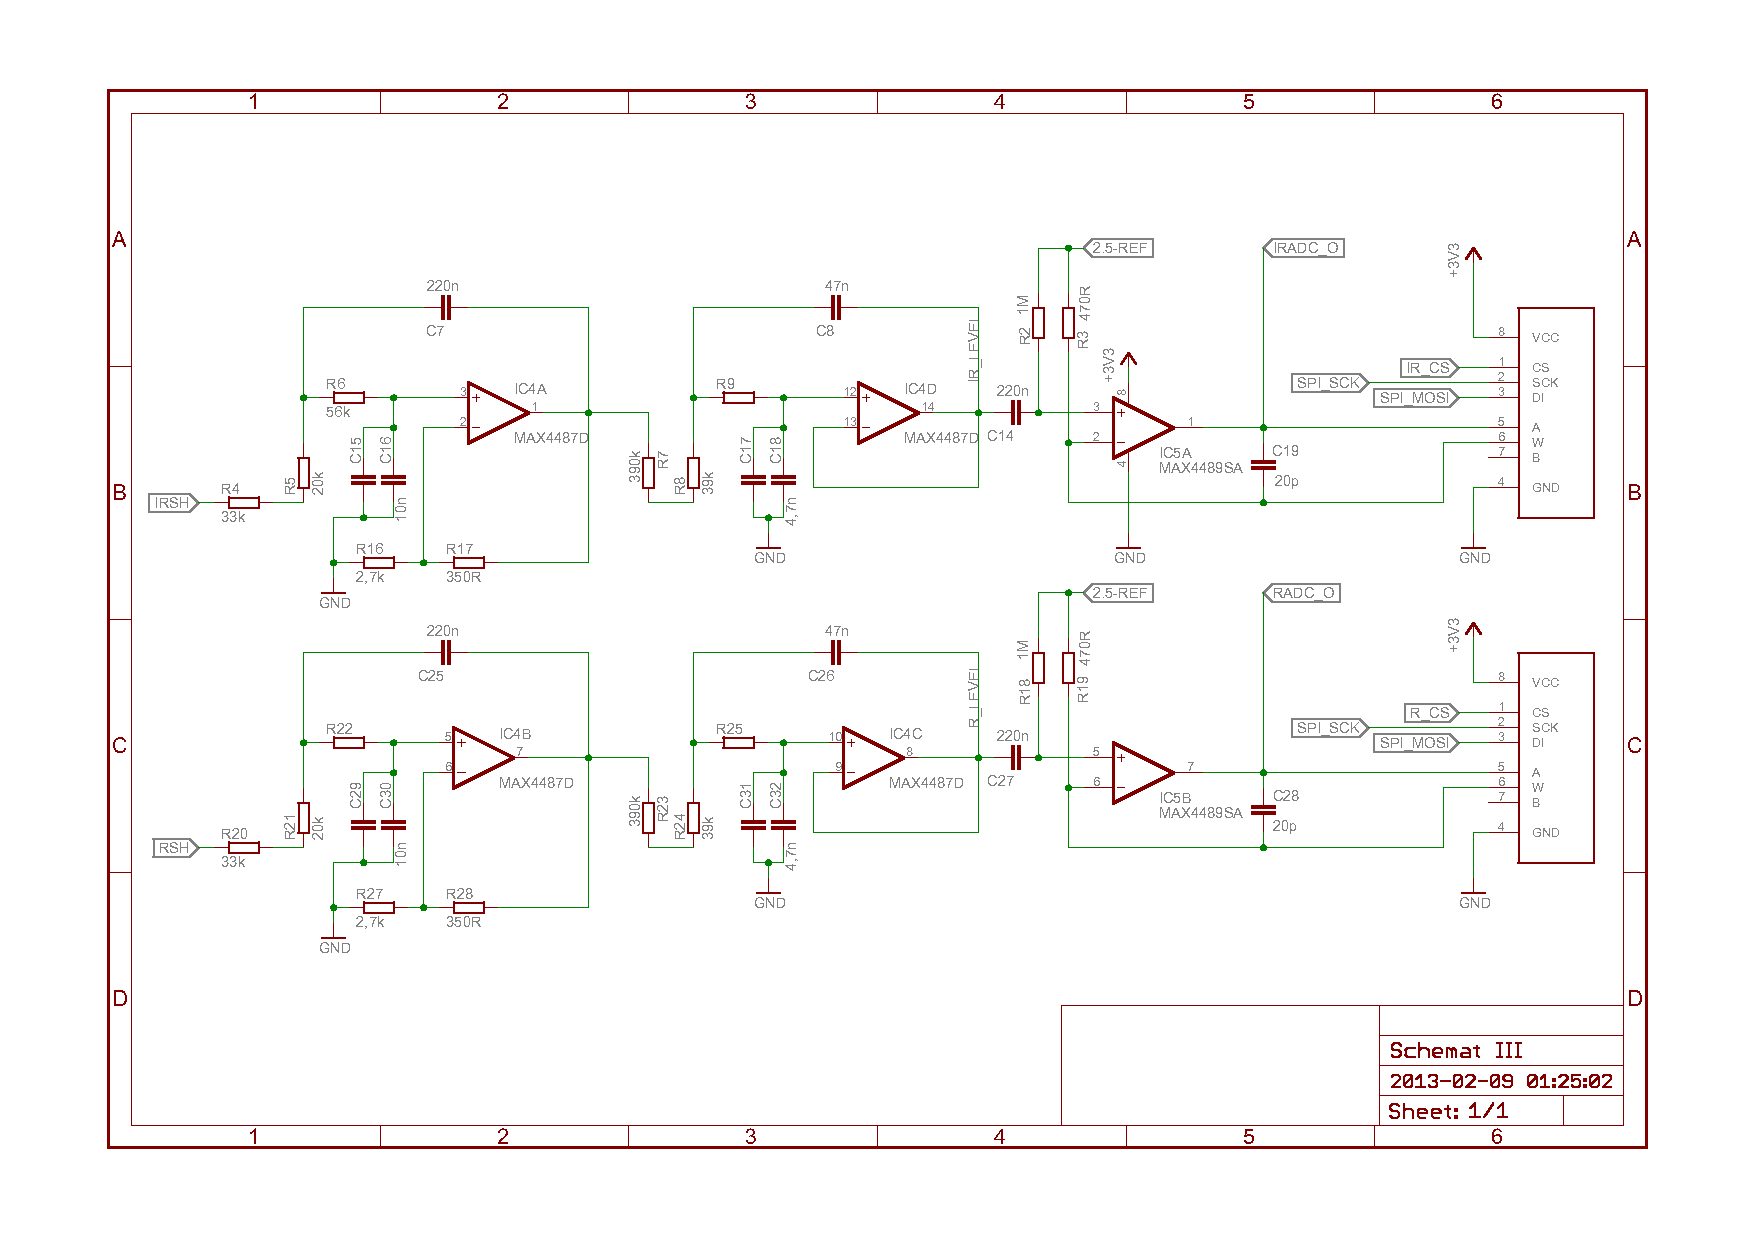
\includepdf[pages={1}, landscape]{graphic/SchematIII.pdf}
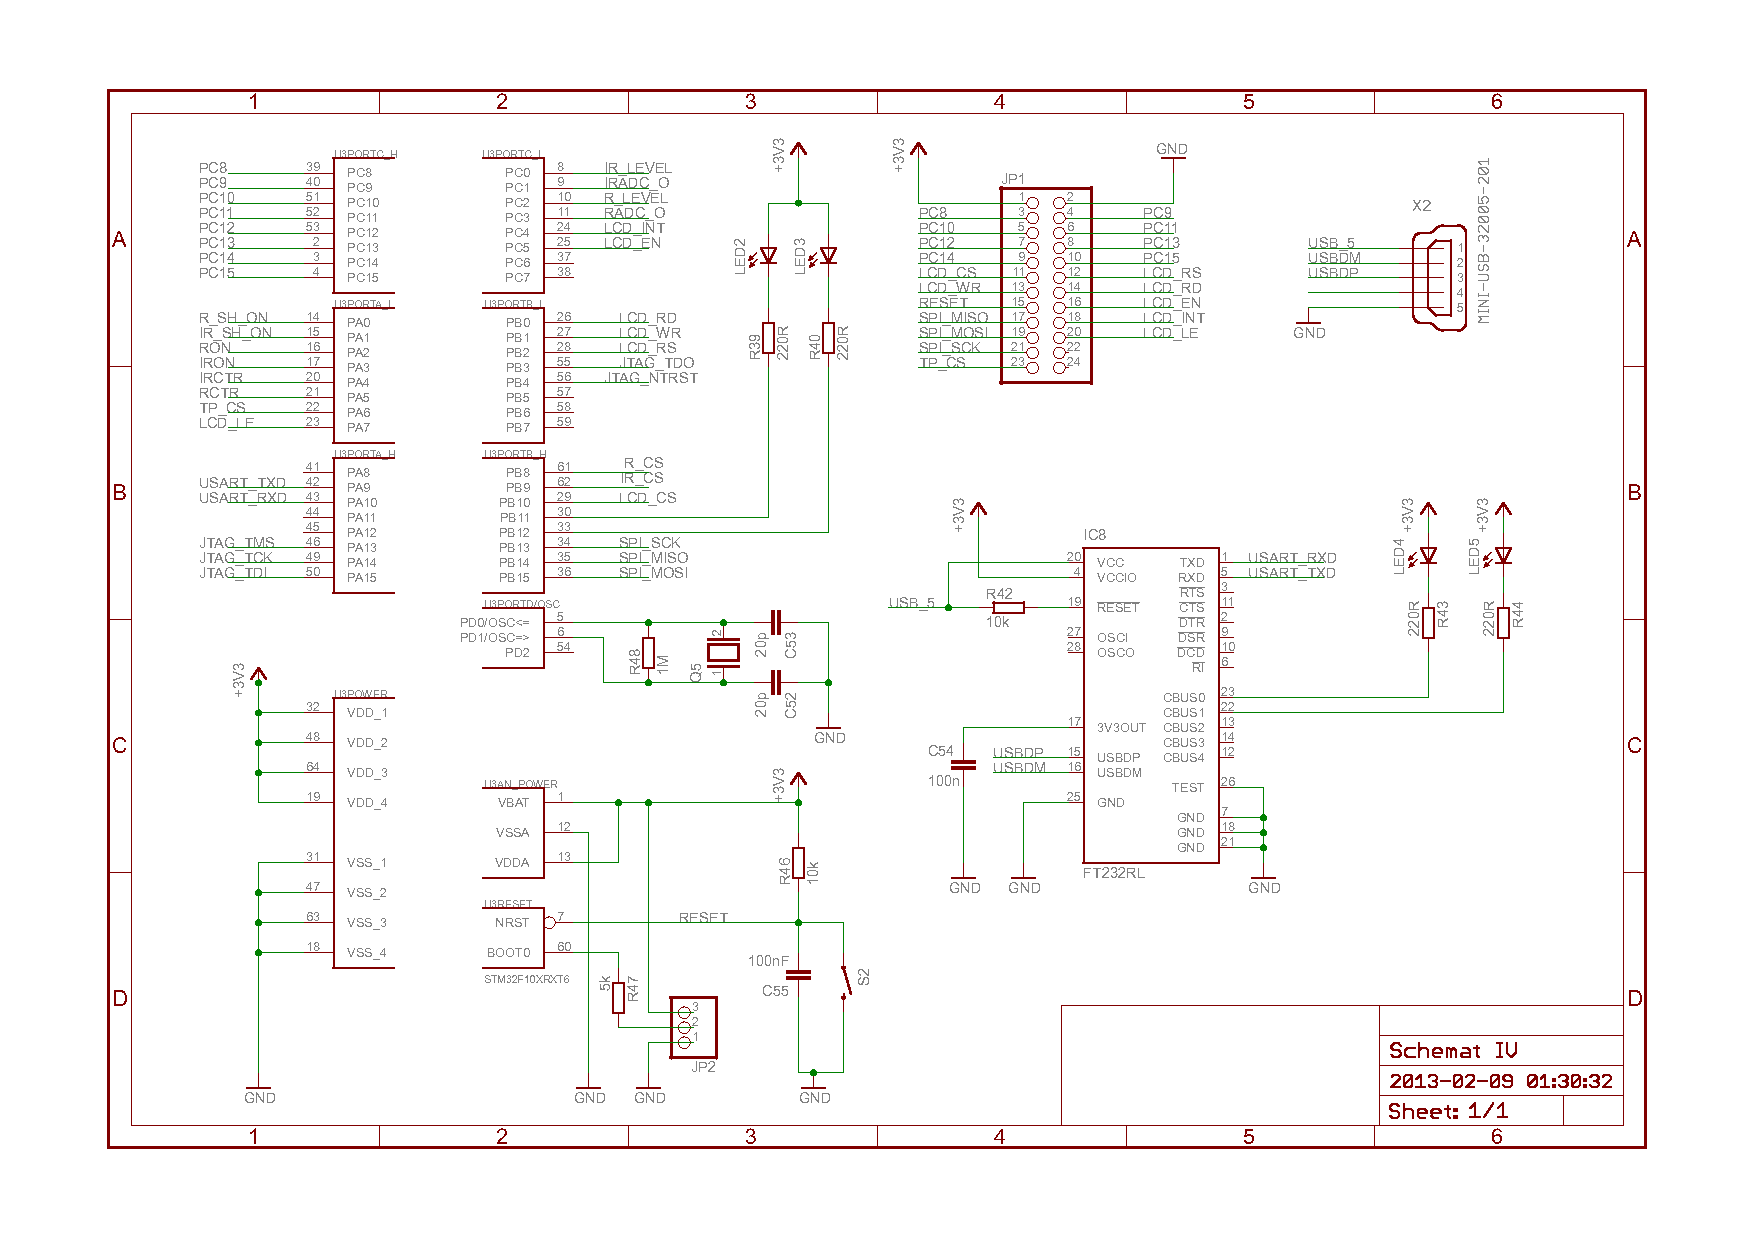
\includepdf[pages={1}, landscape]{graphic/SchematIV.pdf}
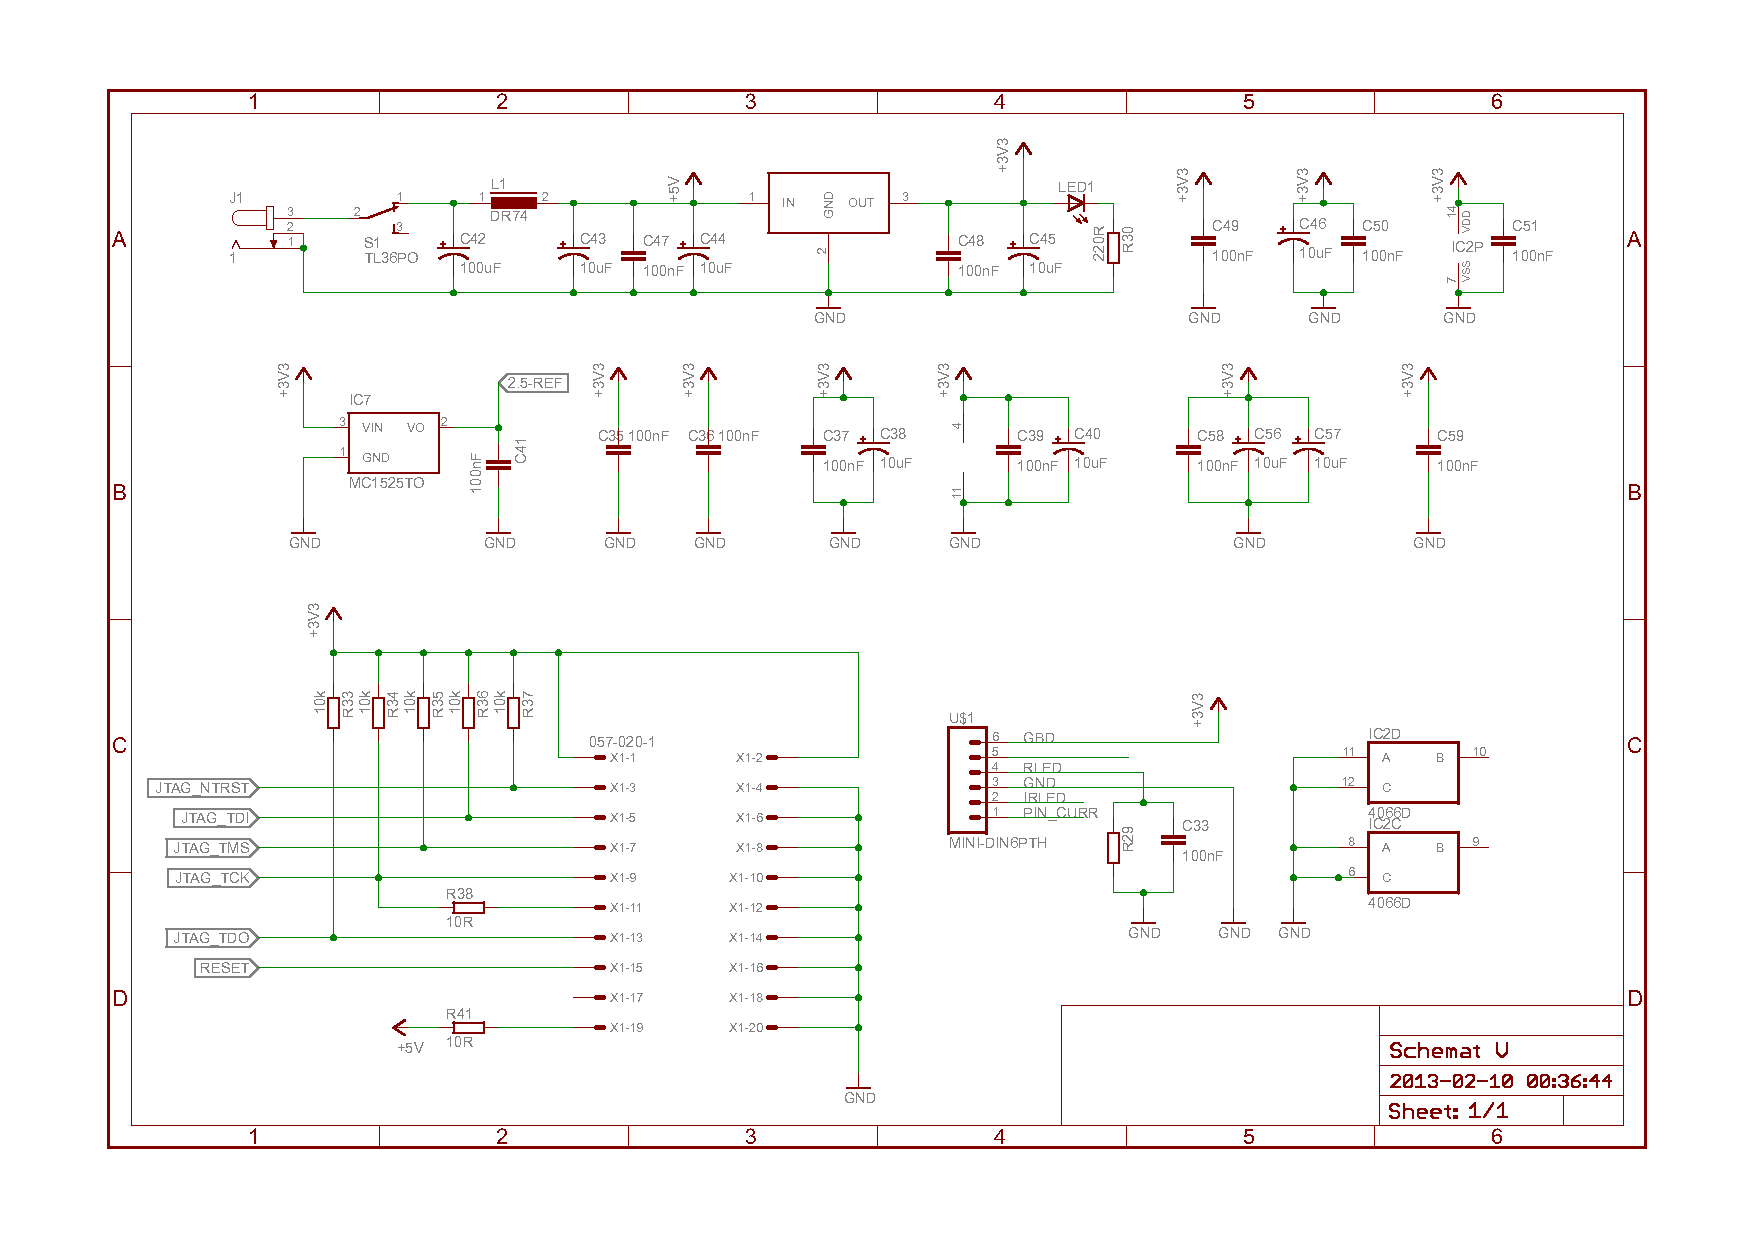
\includepdf[pages={1}, landscape]{graphic/SchematV.pdf}

\newpage
\begin{figure}[!ht]
	\centerline{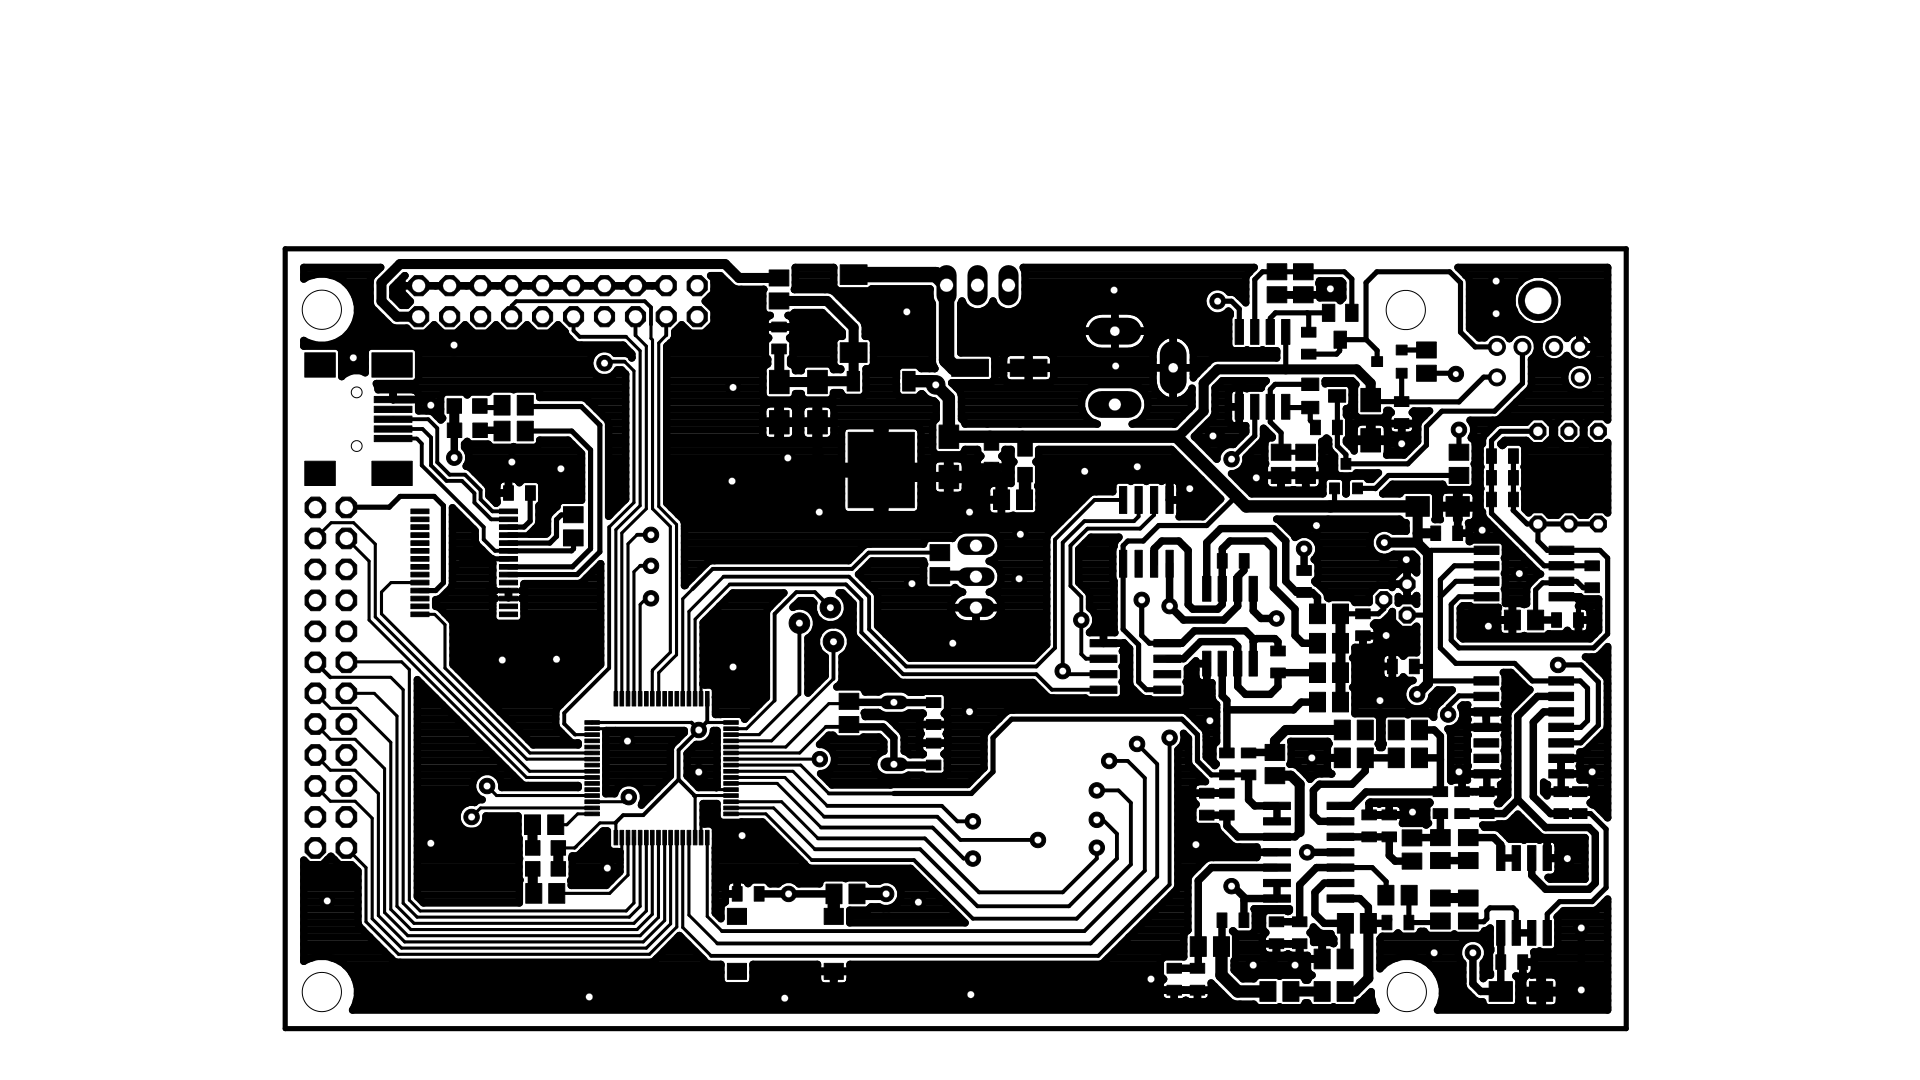
\includegraphics[scale = 0.26]{graphic/top.png}}
	\caption{Warstwa TOP (odbicie lustrzane)}
	\label{rys:Dlon}
\end{figure}
\begin{figure}[!ht]
	\centerline{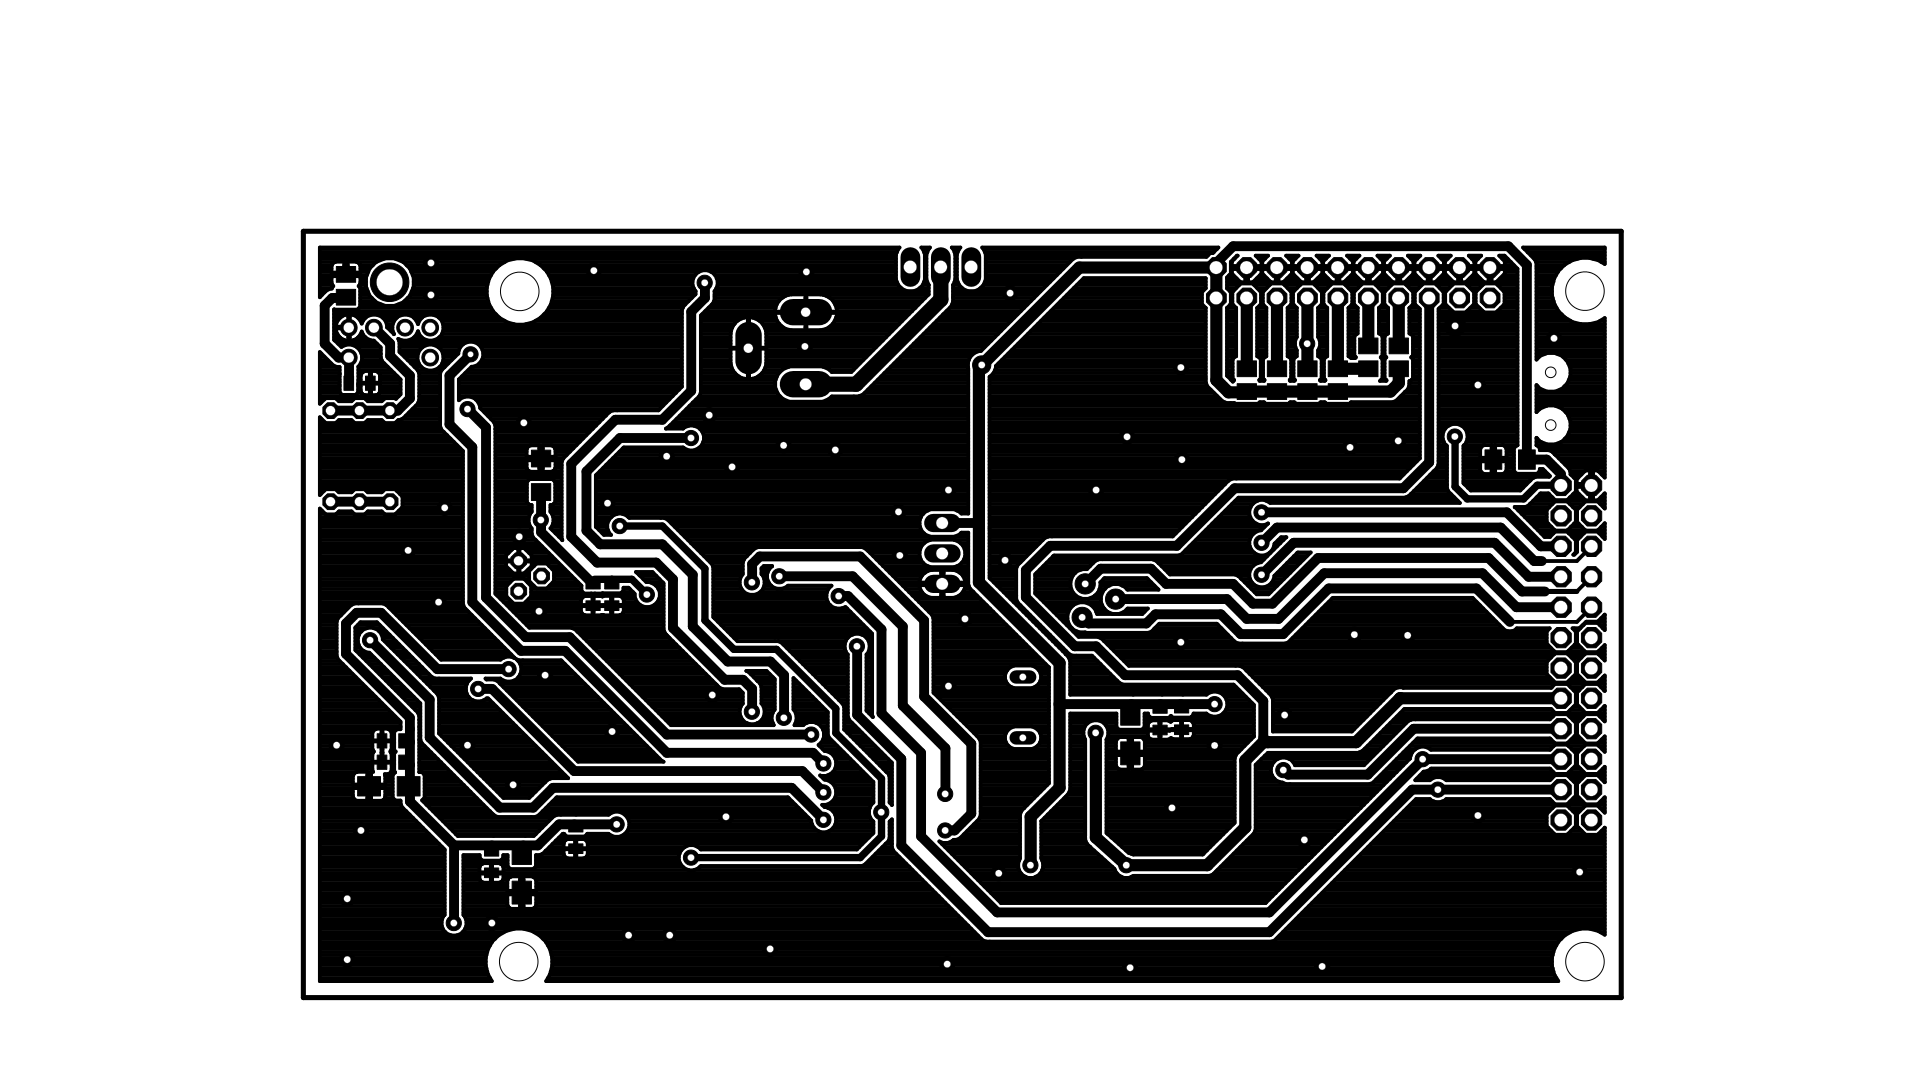
\includegraphics[scale = 0.26]{graphic/bottom.png}}
	\caption{Warstwa BOTTOM}
	\label{rys:Dlon}
\end{figure}
\newpage

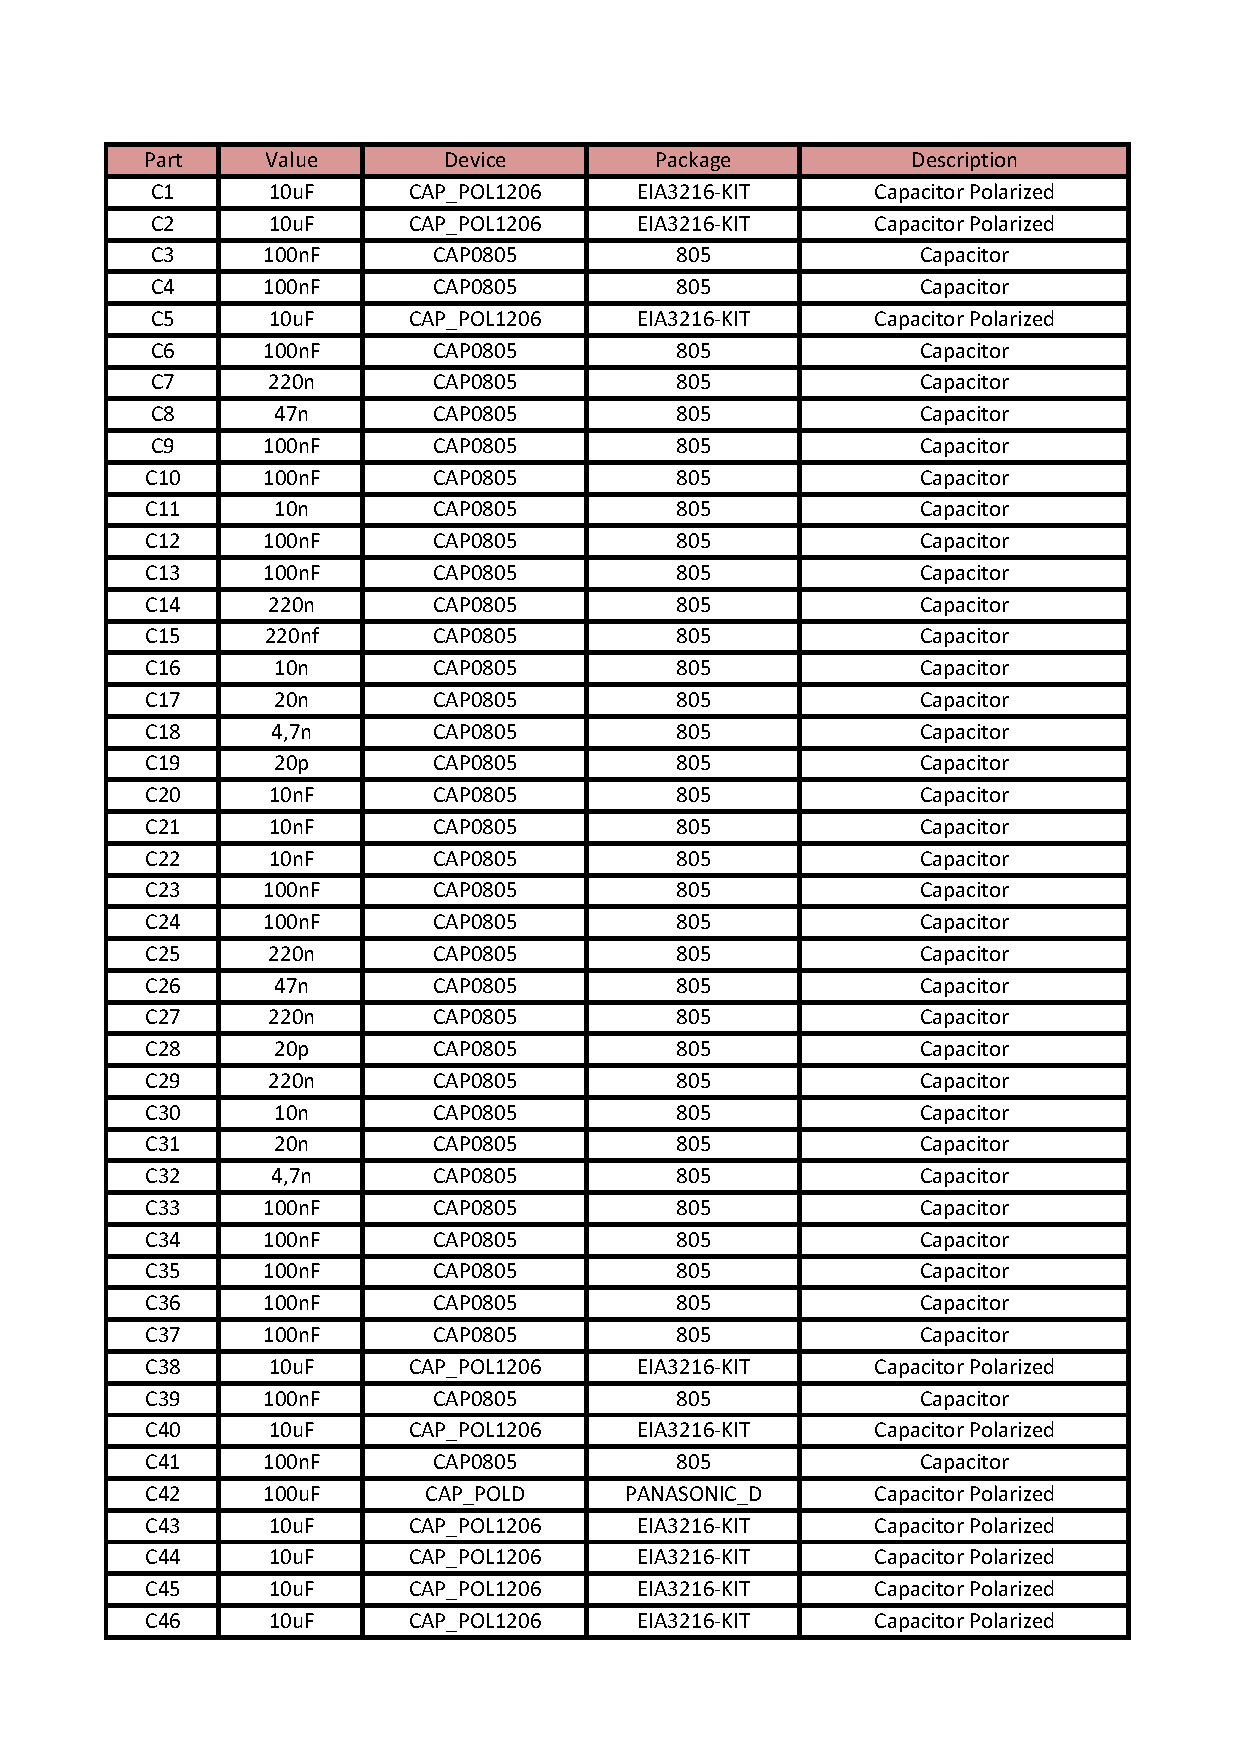
\includepdf[pages={1,2}]{graphic/BOM.pdf}
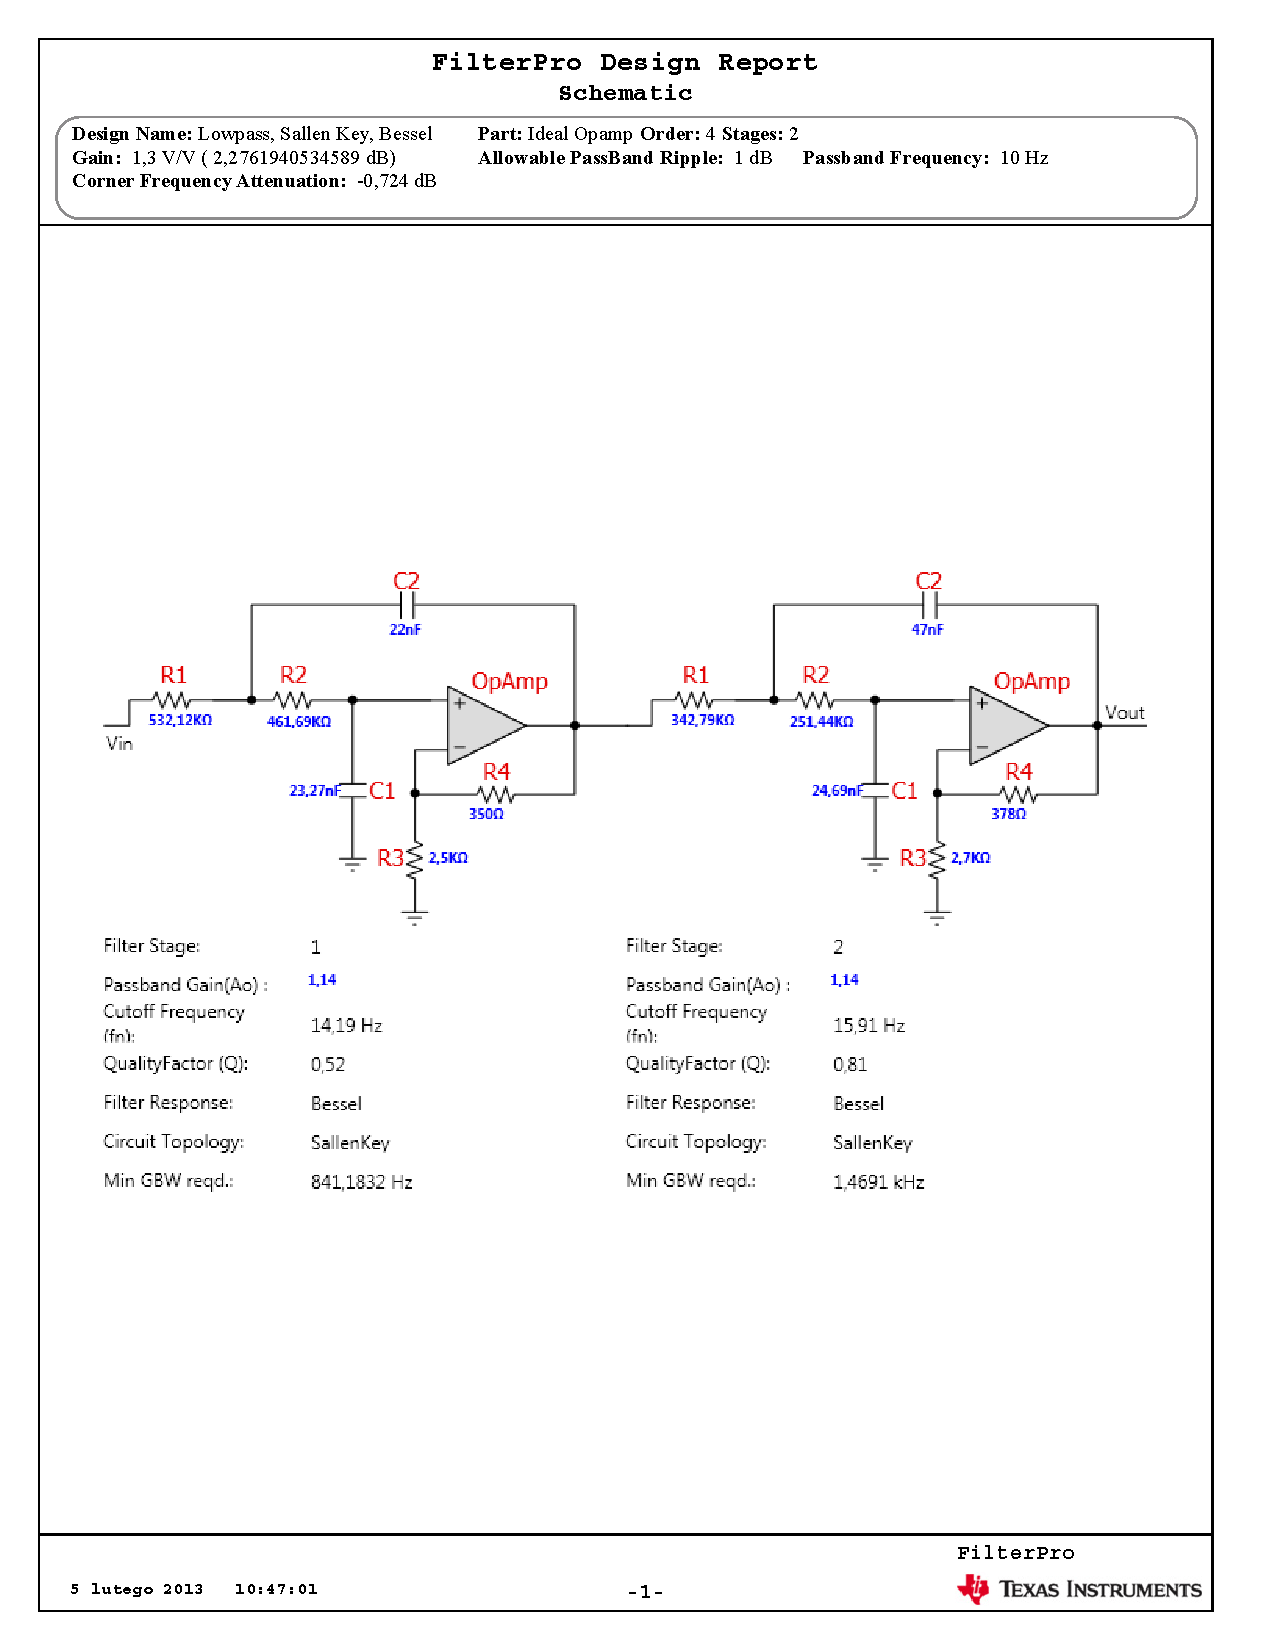
\includepdf[pages={1,2}]{graphic/designreport.pdf}

